\documentclass{beamer} % [handout] para imprimir eliminando transiciones

%\usefonttheme[onlymath]{serif}
%\usepackage{fontspec}
%\defaultfontfeatures{Mapping=tex-text}
%\setsansfont[Ligatures={Common}]{Futura}
%\setmonofont[Scale=0.8]{Monaco} 

\usepackage{beamerthemesplit}
\usepackage[utf8]{inputenc}
\usepackage[spanish]{babel}
\mode<presentation>
\usetheme{default}
\usecolortheme{dolphin}
\usepackage{alltt}                                    % \begin{alltt}
\usepackage{amssymb}                                  % mathematical symbols
\usepackage{comment}
\usepackage{tabto}                                    % \tabto
\usepackage{verbatim}                                 % comentarios

\title{Lenguajes de Programación}                     %[titulo corto]
\author{Fabián Riquelme Csori}                        %[nombre corto]
\date{2017}                                           %[fecha corta]
\institute{Universidad de Valparaíso}                 %[instituto corto]

\newcommand{\HRule}{\rule{\linewidth}{0.2mm}\\[1ex]}
\newcommand{\blue}[1]{\textcolor{blue}{#1}}
\newcommand{\red}[1]{\textcolor{red}{#1}}
\newcommand{\redb}[1]{{\color{red!70!black}{#1}}}
\newcommand{\green}[1]{{\color{green!70!black}{#1}}}
\newcommand{\gray}[1]{{\color{gray!50!white}{#1}}}
\newcommand{\textgreek}[1]{\begingroup\fontencoding{LGR}\selectfont#1\endgroup}
% \alert{texto destacado en rojo}
% \color{green} Color en verde
% \structure{texto en lila}

\begin{document}


%\begin{frame}%[plain]
%  \titlepage
%\end{frame}
%
% [opciones]:
% plain: oculta barra de navegacion, deja + espacio para contenido
% fragile: usar comandos como verbatim
% b,c,t: alineacion vertical
% label=nombre_etiqueta
% allowframebreaks: divide contenido en varios frames si es demasiado largo
% shrink: para escribir mucho texto en una transparencia, reduciendo tamano de fuente

%%%%%%%%%% PORTADA %%%%%%%%%%
\begin{frame}[plain]
  \begin{figure}[h]
    \begin{minipage}{0.3\textwidth}
    
\includegraphics[width=.9\textwidth]{./image/logo-UV.png}
    \end{minipage}
    \begin{minipage}{0.65\textwidth}
     $~$\\[3.6ex]
     \footnotesize{Escuela de Ingeniería Civil Informática}\\
     \footnotesize{Facultad de Ingeniería}
    \end{minipage}
  \end{figure}
  \begin{center}
    \vspace{1ex}
    \HRule
    \Large{Lenguajes de Programación}\\{\small Capítulo I: Lenguajes, compiladores e intérpretes}\\[-1ex]
    \HRule\vspace{1ex}
    \large{Fabián Riquelme Csori}\\[.5ex]\footnotesize{fabian.riquelme@uv.cl}\\[6ex] {\tiny 2017-II}\\[6ex]
  \end{center}
\end{frame}

%%%%%%%%%% INDEX %%%%%%%%%%
\begin{frame}
 \frametitle{Index}
 \scriptsize 			% reducir tamano de letra
 \tableofcontents		%[pausesections]
\end{frame}

%%%%%%%%%%% ACTUAL INDEX %%%%%%%%%%
%\AtBeginSection[] %generar indice automaticamente
%{
%\begin{frame}<beamer>%[plain]
% \frametitle{Index}
% \framesubtitle{subtitulo}
% \scriptsize
% \tableofcontents[currentsection, currentsubsection]
%\end{frame}
%}

%==============================
\section{Introducción}
%------------------------------

%------------------------------
\subsection{Lenguajes de programación}

\begin{frame}{¿Qué lenguajes de programación conoces?}
    \pause
    \begin{center}
    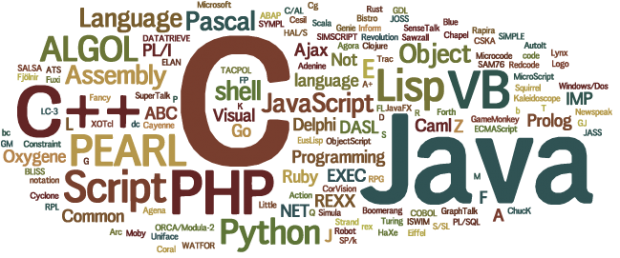
\includegraphics[width=\textwidth]{./image/cap1/languages}
    \end{center}
    \scriptsize{\url{http://spectrum.ieee.org/static/interactive-the-top-programming-languages-2017}}
\end{frame}

\begin{frame}{¿Qué lenguajes se parecen más entre sí?}
    \begin{tabular}{cccl}
      1. & \textsf{a[25]}             & Java       & bounds checking\\
      2. & \textsf{(vector-ref a 25)} & Racket     & bounds checking\\
      3. & \textsf{a[25]}             & C          & no bounds checking\\
      4. & \textsf{a[25]}             & Haskell/ML & función aplicada a una lista\\
    \end{tabular}
\end{frame}

\begin{frame}{¿De qué se trata este curso?}
    Una introducción a los principios fundamentales acerca del diseño, semántica e implementación de lenguajes de programación.
    \begin{block}{Objetivos}
      \begin{itemize}\small{
        \item Conocer distintos paradigmas de programación, así como sus ventajas y desventajas relativas.
        \item Conocer los principios transversales sobre los cuales se diseñan e implementan los lenguajes de programación.
        \item Identificar propiedades de un lenguaje de programación.
        \item Aprender a pensar la solución de un problema en términos abstractos en lugar de hacerlo atado a la sintaxis de un lenguaje en particular.
        \item Estar preparado para nuevos métodos de programación, paradigmas y herramientas.}
      \end{itemize}
    \end{block}
\end{frame}

\begin{frame}{¿Qué es un lenguaje de programación?}
    \begin{block}{Según la RAE}
      \begin{itemize}
        \item \blue{Lenguaje} 7. \textit{Inform}. Conjunto de signos y reglas que permite la comunicación con una computadora.
        \item \alert{\underline{Lenguaje} máquina} 1. \textit{Inform}. Conjunto de instrucciones codificadas que una computadora interpreta y ejecuta directamente.
        \item \blue{Programar} 4. Elaborar programas para su empleo en computadoras.
      \end{itemize}
    \end{block}
    \pause
    \begin{block}{Wikipedia}
    Un lenguaje de programación es un \underline{lenguaje formal} diseñado para realizar \underline{procesos} que pueden ser llevados a cabo por máquinas como las \underline{computadoras}.
    \end{block}
\end{frame}

\begin{frame}{}
    \begin{center}
      
\includegraphics[width=.7\textheight]{./image/cap1/humano-computador}
    \end{center}
\end{frame}

\begin{frame}{¿Por qué estudiar lenguajes de programación?}
    \begin{itemize}
      \item<1-> ¡Simple curiosidad!
      \item<2-> Determinar el lenguaje más apropiado para cierta tarea:
      \begin{itemize}
          \item ¿Computación simbólica?
          \item ¿Programación de sistemas operativos?
          \item ¿Aplicaciones web?
          \item ¿Sistemas embebidos y microcontroladores?
      \end{itemize}
      \item<3-> Entender funcionalidades ``oscuras'': herencia múltiple, clausuras, polimorfismo, generics, templates, auto pointers...
      \item<4-> Buscar maneras alternativas de expresar cosas.
      \item<5-> Hacer mejor uso de la tecnología disponible (TI).
      \begin{itemize}
          \item Existen tecnologías de lenguajes muy presentes en la industria: parsers, JSON, lenguajes sobre Javascript (Coffescript, Dart, TypeScript), lenguajes de plantillas, etc.
      \end{itemize}
    \end{itemize}
\end{frame}

\begin{frame}{¿Por qué estudiar lenguajes de programación?}
    \begin{itemize}
      \item<1-> Para facilitar nuestro aprendizaje de nuevos lenguajes.
      \begin{itemize}
          \item Aprender C\# es más fácil si ya se sabe Java.
          \item Aprender Haskell es más fácil si ya se sabe ML.
          \item Al conocer los principios subyacentes, es más fácil determinar lo que distingue a un lenguaje de otro.
          \item Muchos lenguajes se diferencian mayoritariamente en su sintáxis, pero no en su semántica.
      \end{itemize}
      \item<2-> Evitar reinventar la rueda y adaptarse a los estándares:
      \begin{itemize}
          \item Android requiere Java/Dalvik.
          \item Apple iOS y OSX requieren Objective-C/Swift.
          \item El ecosistema Microsoft requiere de .NET (C\#, F\#, VB.Net).
          \item HTML, CSS y Javascript son el ``assembler'' de la web.
          \item El kernel de Linux está escrito en C.
      \end{itemize}
    \end{itemize}
\end{frame}

%------------------------------
\subsection{Un poco de historia}

\begin{frame}{Lenguaje de máquina}
    En los 1940s se programaba directamente en \blue{lenguaje de máquina}.
    \medskip
    
    \scriptsize{\texttt{\hspace{2ex} 27bdffd0 afbf0014 0c1002a8 00000000 0c1002a8 afa2001c 8fa4001c\\
    \hspace{2ex} 00401825 10820008 0064082a 10200003 00000000 10000002 00832023\\
    \hspace{2ex} 00641823 1483fffa 0064082a 0c1002b2 00000000 8fbf0014 27bd0020\\
    \hspace{2ex} 03e00008 00001025}}
    \medskip

    \scriptsize{Ejemplo de programa para calcular el máximo común denominador GCD($a$,$b$) en lenguaje de máquina Intel x86.}
    \medskip
    
    \pause
    \begin{minipage}{0.47\textwidth}
    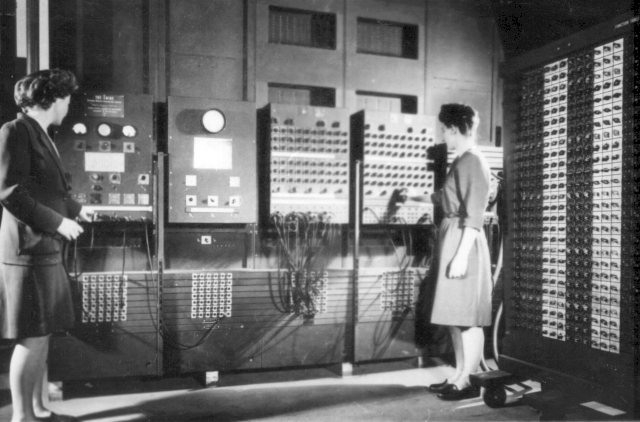
\includegraphics[width=.95\textwidth]{./image/cap1/ENIAC}
    \end{minipage}
    \begin{minipage}{0.52\textwidth}
      \scriptsize{ENIAC y 2 de sus 6 programadoras\\
      \url{https://es.wikipedia.org/wiki/ENIAC}.\\\pause
      El \blue{tiempo de máquina} era mucho más valioso que el \blue{tiempo de implementación} o \blue{desarrollo}.}
    \end{minipage}
\end{frame}

\begin{frame}[fragile=singleslide]{Assembler}
   \begin{itemize}\small{
     \item Un \blue{assembler} (ensamblador) es un lenguaje de bajo nivel.
     \item Son abreviaciones mnemotécnicas con correspondencia (casi) 1 a 1 con el lenguaje máquina.
     \item Creados para diversas arquitecturas desde 1949.}
   \end{itemize}
  
   \scriptsize{\begin{alltt}
        addiu sp,sp,-32
        sw    ra,20(sp)        b      C
        jal   getint           subu   a0,a0,v1
        nop                 B: subu   v1,v1,a0
        jal   getint        C: bne    a0,v1,A
        sw    v0,28(sp)        slt    at,v1,a0
        lw    a0,28(sp)     D: jal    putint
        move  v1,v0            nop
        beq   a0,v0,D          lw     ra,20(sp)
        slt   at,v1,a0         addiu  sp,sp,32
     A: beq   at,zero,B        jr     ra
        nop                    move   v0,zero\end{alltt}}
    \scriptsize{Programación de GCD($a$,$b$) para arquitectura MIPS.}
\end{frame}

\begin{frame}{La historia sigue...}
  \scriptsize{\begin{itemize}
      \item<1-> A medida que aumenta la tecnología, nuevas arquitecturas compiten en el mercado (x86, MIPS, SPARC, ARM).
      \item<2-> Se vuelve tedioso y \red{costoso} crear y mantener software para distintas arquitecturas.
      \item<3-> Se vuelve \red{difícil} (para los humanos) y \red{costoso} crear grandes programas en ensamblador.
      \item<4-> En 1952, Grace Hopper crea A-0 System, el primer \blue{compilador}, para UNIVAC I.
      \item<5-> En 1957, John W. Backus et al. crean un compilador para \blue{FORTRAN} (Formula Translating System), el primer lenguaje de programación de alto nivel, diseñado específicamente para procesamiento de operaciones numéricas.\\
      Se usaron \red{18 años-hombre} para la implementación.
      \item<6-> Surgen nuevos lenguajes y compiladores: \blue{ALGOL}, \blue{COBOL}, \blue{LISP}...
      \item<7-> Entre 1969 y 1973, Dennis Ritchie crea el \blue{lenguaje C}, diseñado para mapear instrucciones de máquina \blue{eficientemente}. Permite usar código en assembler.\\
      Hoy se considera un \blue{assembler portable}.
      \item<8-> C++ aparece en 1983; Python en 1991; Java y PHP en 1995.
      \item<9-> Etc... representación gráfica hasta 2004: \url{http://cdn.oreillystatic.com/news/graphics/prog_lang_poster.pdf}
  \end{itemize}}
\end{frame}

\begin{frame}{La realidad actual}
  \begin{itemize}
    \item<1-> Nuevos avances en hardware (instrucciones MMX, pipelines, GPUs, etc.) hacen aún más difícil la tarea de implementar compiladores que generen código eficiente.
    \item<2-> En general, en la actualidad es muy difícil que un humano pueda generar código ensamblador que sea significativamente más eficiente que el generado por un compilador.
    \item<3-> Además, hoy el \blue{tiempo de máquina} es barato, en comparación con el \red{tiempo de desarrollo}, el \red{costo de los desarrolladores}, y el \red{costo de mantenimiento} del software.
  \end{itemize}
\end{frame}

%==============================
\section{Compiladores e Intérpretes}
%------------------------------
\subsection{Paradigmas de programación}

\begin{frame}{¿Por qué existen tantos lenguajes?}
  \begin{itemize}
    \item<1-> Evolución: a medida que avanza el tiempo, se crean mejores maneras de hacer las cosas.
    \item<2-> Algunos se crearon para propósitos específicos: Lisp, Awk, ¿C?
    \item<3-> Preferencias personales: ¿por qué no inventar mi propio lenguaje? Python, PHP, Ruby.
    \item<4-> Poder expresivo / Poder de abstracción: casi todos los lenguajes son \blue{Turing-completos}, pero no es lo mismo programar una aplicación web en C, que en Ruby (on Rails).
    \item<5-> Facilidad de uso, estandarización, eficiencia, filosofía (open source vs. comercial).
    \item<6-> Factores económicos y patrocinio industrial: Apple (Objective-C), IBM / Oracle (Java), Microsoft (C\#), ...
  \end{itemize}
\end{frame}

\begin{frame}{Paradigmas}
  Un \blue{paradigma de programación} es un estilo de programación que provee mecanismos de \blue{descomposición} y \blue{abstracción} para la creación de programas.
  \medskip\pause
  
  \small{
  \begin{tabular}{p{30ex}p{30ex}}
    \blue{Programación declarativa} & \blue{Programación imperativa}\\
    \blue{$\blacktriangleright$} Funcional
      & \blue{$\blacktriangleright$} ``von Neumann''    \\
    \blue{$\blacktriangleright$} Dataflow
      & \blue{$\blacktriangleright$} Scripting          \\
    \blue{$\blacktriangleright$} Lógica
      & \blue{$\blacktriangleright$} Orientada a objetos\\
    \blue{$\blacktriangleright$} Constrained-based  &   \\
    \blue{$\blacktriangleright$} Template-based     &   \\
    \scriptsize{Programador declara ``qué quiere'', sin especificar el ``cómo''.}
      & \scriptsize{Programador se enfoca en ``cómo'' se implementa/ejecuta el algoritmo.}
  \end{tabular}}
  \medskip\pause
  
  Las distinciones entre paradigmas no están totalmente definidas, y las fronteras son borrosas.\\
  Un lenguaje puede combinar varios paradigmas: Scheme, Scala, C\#...
\end{frame}

\begin{frame}{GCD}
    \begin{center}
      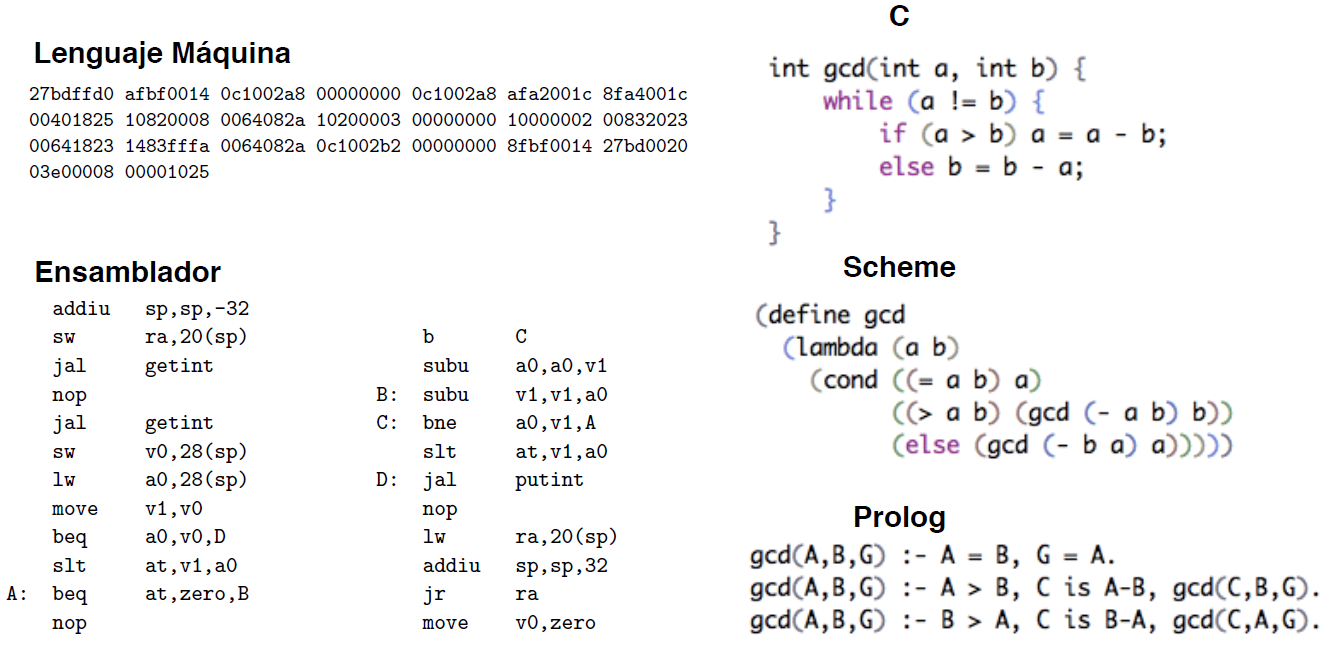
\includegraphics[width=\textwidth]{./image/cap1/GCD}
    \end{center}
\end{frame}

%------------------------------
\subsection{Compilación e interpretación}

\begin{frame}{Compiladores}
    \begin{itemize}
      \item Los computadores sólo entienden lenguaje de máquina.
      \item Un \blue{compilador} es un programa que transforma un lenguaje de alto nivel a ensamblador o lenguaje de máquina.
    \end{itemize}
    \begin{center}
      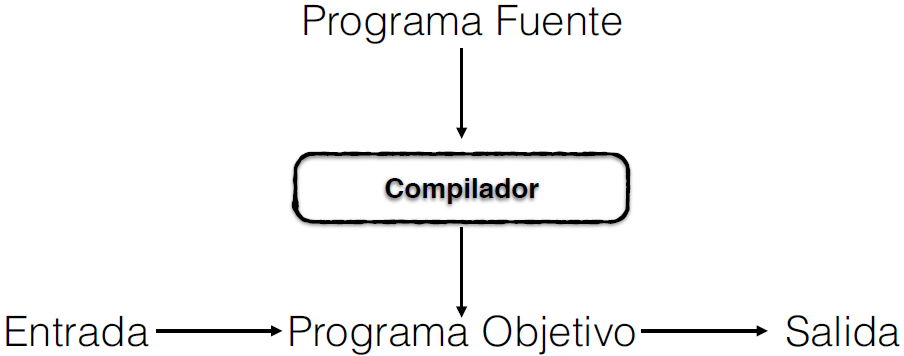
\includegraphics[width=.8\textwidth]{./image/cap1/compilador}
    \end{center}
\end{frame}

\begin{frame}{Compiladores}
    \begin{center}
      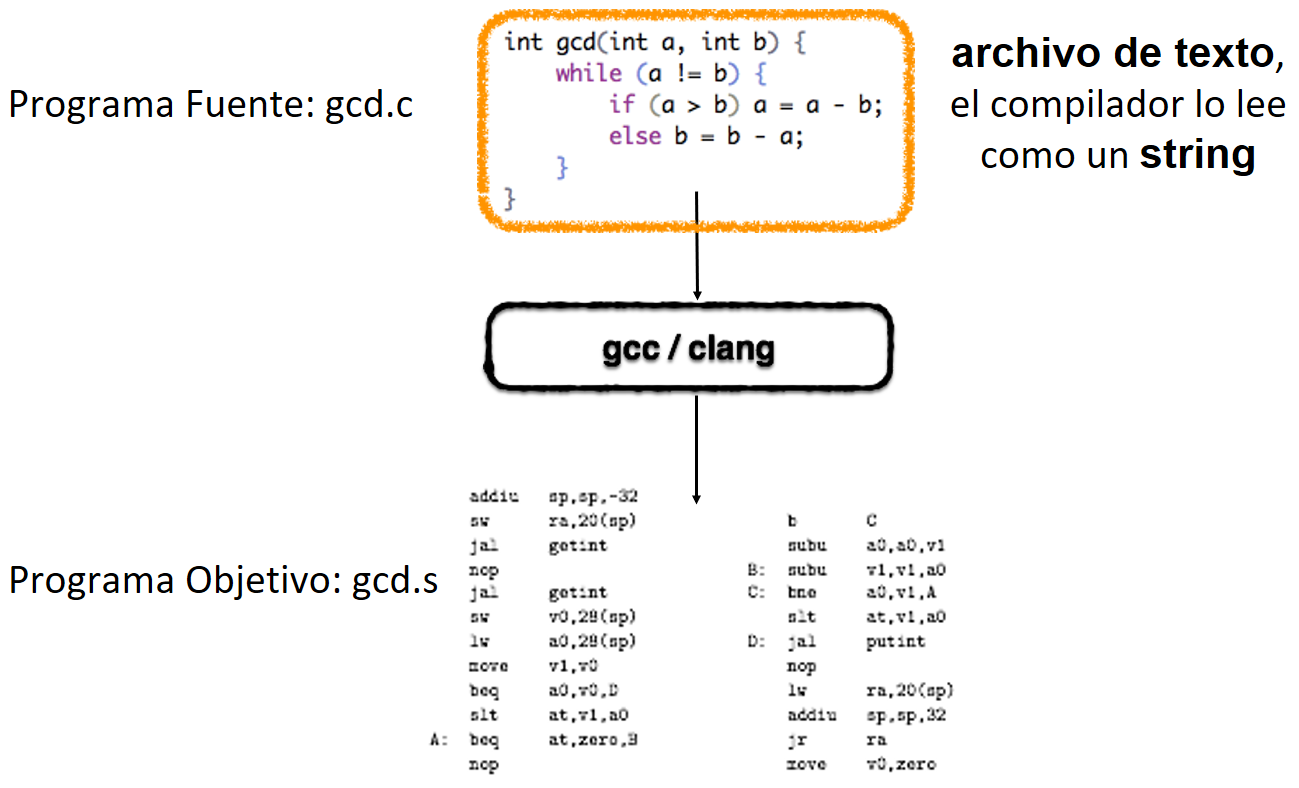
\includegraphics[width=\textwidth]{./image/cap1/compilador-ejemplo}
    \end{center}
\end{frame}

\begin{frame}{Compiladores}
    \begin{itemize}
      \item El compilador transforma el programa fuente en un programa objetivo, típicamente en lenguaje máquina.
      \item Durante la transformación, sólo el compilador está bajo el control de ese proceso. Una vez compilado el programa, el compilador ya no tiene injerencia.
      \item Posteriormente, el usuario pide al sistema operativo que ejecute el programa. El programa controla su propia ejecución sin intervención del compilador.
    \end{itemize}
\end{frame}

\begin{frame}{Intérpretes}
    A diferencia de un compilador, un intérprete sigue presente durante la ejecución de un programa. De hecho, es el actor principal durante la ejecución del mismo.
    \begin{center}
      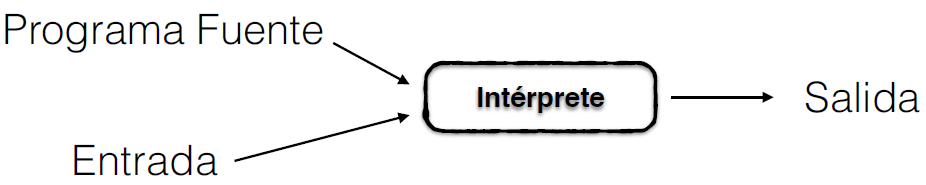
\includegraphics[width=.8\textwidth]{./image/cap1/interprete}
    \end{center}
\end{frame}

\begin{frame}{Intérpretes}
    \begin{itemize}
      \item Un intérprete puede considerarse como una máquina virtual, cuyo lenguaje máquina coincide con el de alto nivel.
      \item En general la interpretación es más flexible que la compilación, por ejemplo dando mejores mensajes de error.
      \item Por otro lado, la compilación en general produce programas con mejor desempeño.
    \end{itemize}
\end{frame}

\begin{frame}{Compilación vs. Interpretación}
    \begin{itemize}
      \item La clasificación de un lenguaje como ``compilado'' o ``interpretado'' no tiene mucho que ver con su semántica.
      \item \textbf{Es posible implementar un intérprete de C, así como es
posible tener un compilador de Python.}
      \item En general, es mejor decir que un lenguaje ``está'' interpretado/compilado, en vez de decir que el lenguaje ``es'' interpretado/compilado.
      \begin{flushright}
      \scriptsize{...En castellano es fácil ver la diferencia entre ``ser'' y ``estar''!}
      \end{flushright}
    \end{itemize}
\end{frame}

\begin{frame}{Enfoques mixtos}
    Muchos lenguajes, entre ellos \blue{Java}, combinan interpretación y compilación.
    \begin{center}
      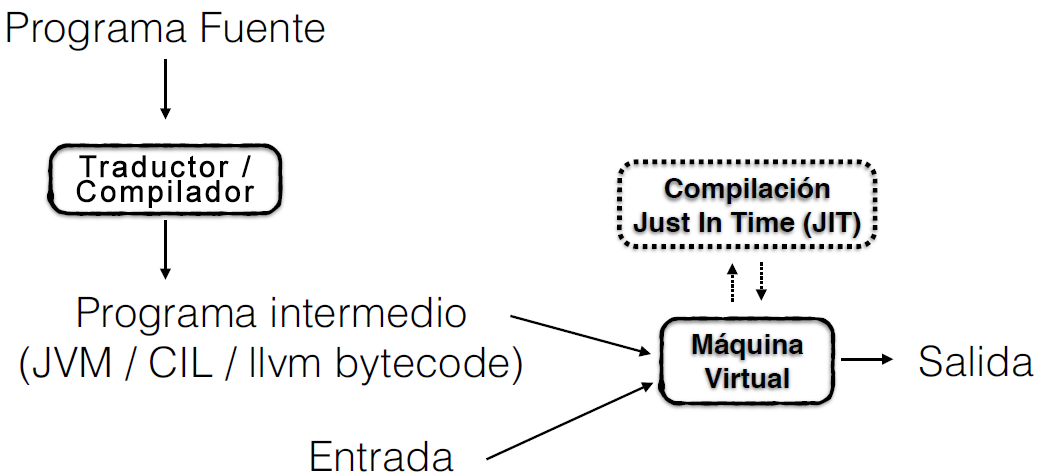
\includegraphics[width=.9\textwidth]{./image/cap1/enfoque-mixto}
    \end{center}
\end{frame}

\begin{frame}{Fases de compilación}
    \begin{itemize}
        \item Un compilador procesa un archivo a través de una serie de \blue{fases} (\textit{compiler phases}), bien definidas.
        \item Cada fase \blue{descubre información} útil para las fases posteriores, o bien \blue{transforma el programa} en una forma que facilita el trabajo de la fase siguiente.
    \end{itemize}
\end{frame}

\begin{frame}{Fases de compilación}
    \begin{center}
      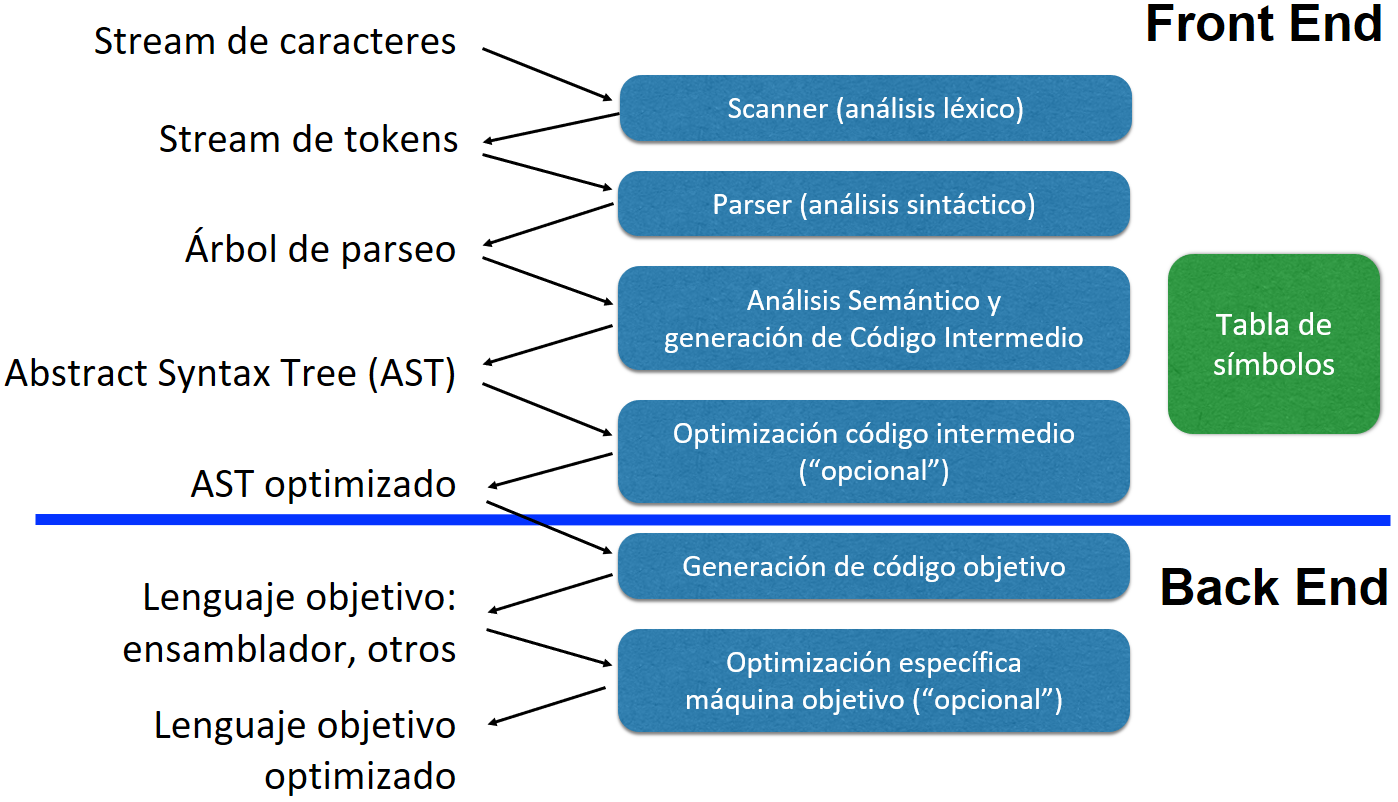
\includegraphics[width=\textwidth]{./image/cap1/compilador-fases}
    \end{center}
\end{frame}

\begin{frame}{Fases de compilación}
    \begin{itemize}
        \item<1-> El \blue{Front End} es independiente del lenguaje objetivo.
        \begin{itemize}
            \item Su objetivo es \blue{capturar el significado} de un programa en el lenguaje fuente.
        \end{itemize}
        \item<2-> El \blue{Back End} es específico para cada lenguaje o máquina objetivo.
        \begin{itemize}
            \item Su objetivo es \blue{generar un programa objetivo equivalente al programa fuente}.
        \end{itemize}
    \end{itemize}
\end{frame}

\begin{frame}{Compiladores en el mundo real}
    \begin{itemize}
        \item<1-> \blue{GCC}
        \begin{itemize}
            \item Front end: C/C++, Objective-C, Ada, Fortran, Java, Go...
            \item Back end: \url{https://gcc.gnu.org/backends.html}
        \end{itemize}
        \item<2-> \blue{LLVM}: \url{http://llvm.org/Features.html}
        \item<3-> \blue{Java JDK}
        \begin{itemize}
            \item El bytecode (.class) es el producto final del Front End.
            \item El Java Runtime Environment (JRE) es la puerta de entrada del Back End.
        \end{itemize}
    \end{itemize}
\end{frame}

%------------------------------

\begin{frame}
 \begin{block}{Bibliografía}
  \begin{itemize}
    \item Pratt, Terrence W. (1998). \textit{Lenguajes de programación: diseño e implementación}, Pearson Education.
    \item Sethi, Ravi (1992). \textit{Lenguajes de programación: conceptos y constructores}, Addison-Wesley Iberoamericana.
    \item Scott, Michael (2009). \textit{Programming Language Pragmatics}, Morgan Kaufman, 3ra ed.
  \end{itemize}
 \end{block}
 \begin{block}{Recursos}
  \begin{itemize}
    \item Apuntes de cursos anteriores (Ismael Figueroa).
    \item Wikipedia y Wikimedia Commons.
    \item Imágenes con licencia libre.
  \end{itemize}
 \end{block}
\end{frame}

\end{document}
